\setcounter{chapter}{3}
\chapter*{Chapter (3): System Architecture}
\addcontentsline{toc}{chapter}{Chapter (3): System Architecture}
\setcounter{section}{0}

\section{Chapter Preview}
This chapter presents the architectural blueprint of the Sanad system. It introduces the high-level hardware-software component layout, details the layered model that decouples core robotics from presentation interfaces, describes the ROS 2 middleware, and traces the lifecycle of a command flow.

\section{System Overview}
\label{sec:arch_overview}

Chapters~1 and~2 established \emph{why} Sanad exists and \emph{what} it must do: replace manual, open-loop wheelchair control with autonomous, goal-directed navigation, driven by an accessibility-first set of input modalities and supported by smart-home and communication features. This chapter answers the next question --- \emph{how the system is put together} --- before Chapters~4 through~11 descend into the implementation of each individual subsystem.

Figure~\ref{fig:system_overview_full} shows every major hardware and software component of Sanad on a single page, deliberately stripped of internal detail. Its only purpose is to give the reader a mental map of the system before the rest of this chapter, and the rest of this book, zooms into each block in turn.

\begin{figure}[H]
\centering
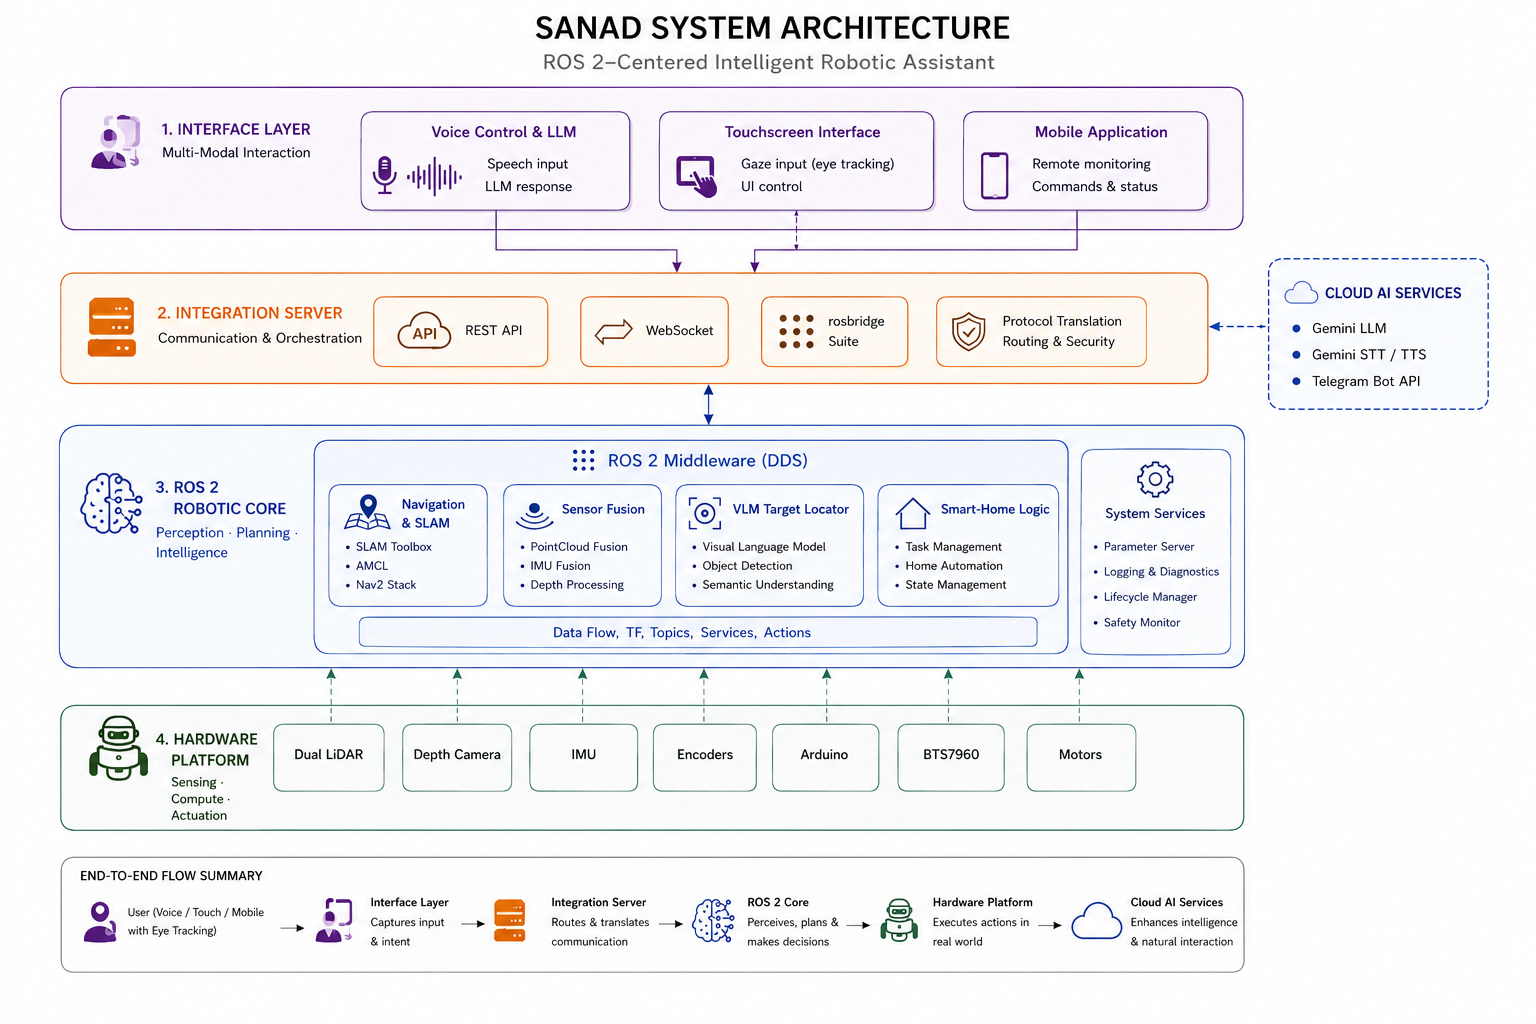
\includegraphics[width=\textwidth]{figures/ch03/system_archtict.png}
\caption{High-level overview of the Sanad system, showing all major hardware and software components organized around the central SANAD Integration Server. Each block is expanded in the corresponding subsystem chapter.}
\label{fig:system_overview_full}
\end{figure}

At a glance, Sanad is composed of five groups of components:

\begin{itemize}
    \item \textbf{Interface Layer} --- five parallel input channels (voice, touchscreen, eye tracking, mobile app, IMU head-tilt) through which a user or caregiver expresses intent, covered in Chapters~5, 7, 8, and~9.
    \item \textbf{Integration Server} --- a single Node.js service that translates between web-facing protocols (REST, WebSocket) and the robot's internal ROS~2 messaging, detailed in Chapter~6.
    \item \textbf{Robotic Core (ROS~2)} --- the autonomous decision-making and motion layer: navigation and SLAM, the voice/LLM intent router, VLM-based target location, and smart-home/communication logic, covered in Chapters~4 and~5.
    \item \textbf{Hardware Platform} --- the physical sensor suite and actuation subsystem that let the robot perceive and move through the world, covered in Chapter~10.
    \item \textbf{Cloud AI Services} --- external, network-dependent services (Gemini LLM, Gemini speech synthesis/recognition, the Telegram Bot API) that the Integration Server calls out to, with a local edge fallback discussed in Chapter~5.
\end{itemize}

The remaining sections of this chapter explain the architectural reasoning that ties these groups together, then walk a single command through the full stack end-to-end.

\section{Layered Architectural Model}
\label{sec:arch_layers}

Rather than a monolithic program, Sanad is organized as four stacked layers, each with a single, well-defined responsibility and a narrow interface to its neighbors. This separation --- expanded on for the server specifically in Section~6.1.3 using a SCADA analogy --- is applied here to the system as a whole, so that presentation-layer changes (e.g., a new mobile screen) never require touching motion-control code, and vice versa.

\begin{figure}[H]
\centering
\begin{tikzpicture}[
    font=\sffamily\small,
    layer/.style={draw=black!60, rounded corners=3pt, thick, minimum width=11.5cm,
        minimum height=1.5cm, align=left, text width=8.6cm, inner sep=8pt, drop shadow},
    tag/.style={draw=black!60, fill=white, rounded corners=2pt, font=\sffamily\scriptsize,
        minimum width=2.6cm, align=center, thick}
]

\node[layer, fill=violet!12, draw=violet!70!black] (l1) at (0,4.5)
    {\textbf{Interface / Presentation Layer}\\[2pt]
     \footnotesize Voice, touchscreen, eye tracking, mobile app, IMU head-tilt --- how the user expresses intent.};

\node[layer, fill=orange!12, draw=orange!70!black, below=0.45cm of l1] (l2)
    {\textbf{Integration / Supervisory Layer}\\[2pt]
     \footnotesize Node.js server: protocol translation, request routing, and rosbridge mediation.};

\node[layer, fill=blue!10, draw=blue!60!black, below=0.45cm of l2] (l3)
    {\textbf{Robotic Middleware Layer (ROS~2)}\\[2pt]
     \footnotesize Navigation, SLAM, sensor fusion, voice/LLM intent router, VLM target locator.};

\node[layer, fill=teal!10, draw=teal!70!black, below=0.45cm of l3] (l4)
    {\textbf{Physical / Field Layer}\\[2pt]
     \footnotesize Sensors (LiDAR, camera, IMU, encoders) and actuation (Arduino, motor drivers).};

\node[tag, right=0.9cm of l1] {Presentation\\(HMI)};
\node[tag, right=0.9cm of l2] {Supervisory};
\node[tag, right=0.9cm of l3] {Control};
\node[tag, right=0.9cm of l4] {Field};

\draw[-{Stealth[scale=0.9]}, thick, draw=gray!60] (l1.south) -- (l2.north);
\draw[-{Stealth[scale=0.9]}, thick, draw=gray!60] (l2.south) -- (l3.north);
\draw[-{Stealth[scale=0.9]}, thick, draw=gray!60] (l3.south) -- (l4.north);

\end{tikzpicture}
\caption{The four-layer architectural model of Sanad, adapted from a SCADA-style stratification of responsibilities (see also Section~6.1.3).}
\label{fig:layered_architecture}
\end{figure}

Two design rules follow directly from this layering. First, \textbf{no layer may skip its neighbor}: a touchscreen button never talks to a ROS~2 node directly, and a navigation node never renders UI --- every cross-layer interaction is mediated by the Integration Server. Second, \textbf{ROS~2 is treated as the boundary of real-time responsibility}: everything at or below the Robotic Middleware Layer must tolerate hard timing constraints (control loops, sensor rates), while everything above it may be arbitrarily delayed by network conditions without endangering the robot, since motion always degrades safely (Chapter~4 covers the relevant safety behaviors).

\section{Hardware Platform}
\label{sec:arch_hardware}

At the base of the stack sits the physical wheelchair platform: a retrofitted manual chair carrying a dual 2D LiDAR array, a depth camera, a chassis IMU, quadrature wheel encoders, and a differential-drive actuation system built around BTS7960 motor drivers and an Arduino running a closed-loop PID velocity controller. An onboard computer runs the ROS~2 graph and communicates with the Arduino over a serial link using the \texttt{SanadInterface} protocol. This chapter treats the hardware platform as a single opaque block (the \textit{Sensor Suite} and \textit{Actuation Subsystem} in Figure~\ref{fig:system_overview_full}); the physical modifications, mechanical calculations, PID tuning, and circuit design are covered in full in Chapter~10.

\section{Robotic Middleware: The ROS~2 Core}
\label{sec:arch_ros2core}

The Robotic Middleware Layer is where perception turns into motion. It is implemented entirely as a graph of ROS~2 nodes communicating over topics, services, and actions, which gives Sanad two properties that matter for a safety-relevant assistive device: individual nodes (say, the VLM target locator) can crash or restart without taking down navigation, and the same navigation stack developed and tested in isolation can be driven by any of the five interface channels without modification. Four functional groups make up this core:

\begin{itemize}
    \item \textbf{Navigation \& SLAM} --- sensor preprocessing, EKF-based odometry fusion, SLAM Toolbox/AMCL localization, Nav2 path planning, and trajectory control (Chapter~4).
    \item \textbf{Voice \& LLM Intent Router} --- wake-word detection, speech-to-text, LLM-based intent parsing, and action routing to the correct subsystem (Chapter~5).
    \item \textbf{VLM Target Locator} --- combines the depth camera with a vision-language model to resolve free-text destinations (``next to the fridge'') into navigable coordinates (Chapter~4, Section~4.13).
    \item \textbf{Smart-Home \& Communication} --- IR blaster control and the autonomous Telegram messaging pipeline, exposed to ROS~2 via the same node-based pattern (Chapters~6 and~9).
\end{itemize}

\section{Integration Server \& Client-Server Communication}
\label{sec:arch_server}

Because ROS~2 is optimized for tightly coupled internal communication rather than heterogeneous external clients, Sanad places a single custom Node.js server between the Robotic Middleware Layer and every client above it. The server exposes a stateless REST API for discrete requests, a persistent WebSocket channel for high-frequency motion telemetry, and a dedicated \texttt{rosbridge} integration layer that multiplexes all ROS-facing communication through one supervised connection with automatic teardown-and-rebuild recovery on disconnect. This dual-server, single-bridge design --- along with the feature-module organization of IR control, Telegram integration, and telemetry --- is the subject of Chapter~6 in full.

\section{Multi-Modal Interface Layer}
\label{sec:arch_interfaces}

Sanad deliberately exposes the \emph{same} underlying capabilities (navigation, smart-home control, communication) through five independent front ends, so that a user's degree of residual physical ability determines which channel they use, not which features they can access. Voice control (Chapter~5) is the primary channel, built on a cloud-first, edge-fallback pipeline with Arabic-language support. The touchscreen (Chapter~7) offers a faster alternative for users with partial hand mobility. Eye tracking (Chapter~8) provides gaze-dwell interaction for users with no reliable speech or limb control. The mobile app (Chapter~9) targets caregivers, providing remote monitoring, biometric alerts, and Telegram-based communication. IMU-based head-tilt sensing (Chapter~4, Section~4.12) adds fine, low-speed maneuvering once a room has been reached. All five channels converge on the same Integration Server endpoints described in Section~\ref{sec:arch_server}, so no channel has privileged or duplicated access to robot behavior.

\section{End-to-End Command Flow: A Worked Example}
\label{sec:arch_e2e}

The clearest way to see the layers of Section~\ref{sec:arch_layers} cooperate is to trace one command through all of them. Figure~\ref{fig:e2e_flow} follows the spoken instruction ``take me to the kitchen'' from utterance to physical motion and back to spoken confirmation.

\begin{figure}[H]
\centering
\begin{tikzpicture}[
    >=Latex,
    font=\sffamily\small,
    x=1cm,
    y=1cm
]

%------------------------------------------------
% Participants
%------------------------------------------------
\node[draw=violet!70!black,fill=violet!10,
rounded corners=3pt,
minimum width=3.2cm,
minimum height=0.75cm,
font=\bfseries] (ui) at (0,0)
{Interface Layer};

\node[draw=orange!70!black,fill=orange!10,
rounded corners=3pt,
minimum width=3.2cm,
minimum height=0.75cm,
font=\bfseries] (server) at (4.2,0)
{Integration Server};

\node[draw=blue!70!black,fill=blue!10,
rounded corners=3pt,
minimum width=3.2cm,
minimum height=0.75cm,
font=\bfseries] (ros) at (8.4,0)
{ROS 2 Core};

\node[draw=teal!70!black,fill=teal!10,
rounded corners=3pt,
minimum width=3.2cm,
minimum height=0.75cm,
font=\bfseries] (hw) at (12.6,0)
{Hardware Platform};

%------------------------------------------------
% Lifelines
%------------------------------------------------
\foreach \x in {0,4.2,8.4,12.6}
{
    \draw[dashed,gray!60] (\x,-0.45)--(\x,-10);
}

%------------------------------------------------
% Messages
%------------------------------------------------

%1
\draw[->,thick,violet!80!black]
(0,-1)--(4.2,-1)
node[midway,above,font=\scriptsize,align=center]
{1. Voice Command\\``Take me to the kitchen''};

%2
\draw[->,thick,orange!80!black]
(4.2,-2)--++(0.9,0)
--++(0,-0.7)
--(4.2,-2.7);

\node[anchor=west,font=\scriptsize]
at (5.2,-2.35)
{2. Speech-to-Text + LLM Intent Parsing};

%3
\draw[->,thick,orange!80!black]
(4.2,-3.2)--++(0.9,0)
--++(0,-0.7)
--(4.2,-3.9);

\node[anchor=west,font=\scriptsize]
at (5.2,-3.55)
{3. Action Intent Router};

%4
\draw[->,thick,orange!80!black]
(4.2,-4.8)--(8.4,-4.8)
node[midway,above,font=\scriptsize]
{4. Navigation Goal (Nav2 Action)};

%5
\draw[->,thick,blue!80!black]
(8.4,-5.7)--++(0.9,0)
--++(0,-0.7)
--(8.4,-6.4);

\node[anchor=west,font=\scriptsize]
at (9.4,-6.05)
{5. Global/Local Planning\\SLAM Toolbox + AMCL};

%6
\draw[->,thick,blue!80!black]
(8.4,-7.2)--(12.6,-7.2)
node[midway,above,font=\scriptsize]
{6. Velocity Commands ($cmd\_vel$)};

%7
\draw[->,thick,teal!80!black]
(12.6,-8)--++(0.9,0)
--++(0,-0.7)
--(12.6,-8.7);

\node[anchor=west,font=\scriptsize]
at (13.6,-8.35)
{7. Closed-loop PID Control};

%8
\draw[<-,thick,blue!80!black]
(4.2,-9.5)--(8.4,-9.5)
node[midway,above,font=\scriptsize]
{8. Goal Reached};

%9
\draw[<-,thick,violet!80!black]
(0,-10)--(4.2,-10)
node[midway,above,font=\scriptsize]
{9. Spoken Confirmation (Gemini TTS)};

\end{tikzpicture}

\caption{Sequence diagram illustrating the end-to-end execution of a voice navigation command across the Sanad software architecture.}
\label{fig:e2e_flow}
\end{figure}

Three properties of this flow are worth highlighting because they recur throughout the rest of the book. First, the request crosses the Interface--Integration--Core boundary exactly once in each direction (steps~3 and~7), consistent with the no-skipping rule of Section~\ref{sec:arch_layers}. Second, once the Navigation Goal is accepted in step~4, the robot completes steps~4--6 autonomously and in a hard real-time loop, entirely independent of network conditions --- if the voice channel that issued the command drops, the chair still safely reaches its destination. Third, the same eight-step shape applies almost unchanged to the other four interface channels; only step~1--2 differs (a touchscreen tap or a gaze-dwell selection replaces speech recognition), which is precisely what allows Section~\ref{sec:arch_interfaces}'s five channels to share one navigation implementation.

\section{Chapter Roadmap}
\label{sec:arch_roadmap}

Table~\ref{table:chapter_roadmap} maps each architectural block introduced in this chapter to the chapter that covers its implementation in detail.

\begin{table}[H]
\centering
\caption{Mapping from architectural layer/component to the chapter covering its implementation.}
\begin{tabular}{|p{4.2cm}|p{6.3cm}|p{2.3cm}|}
\hline
\textbf{Layer} & \textbf{Component} & \textbf{Chapter} \\
\hline
\multirow{4}{4.2cm}{Interface Layer} & Voice Control \& LLM & 5 \\
\cline{2-3}
 & Touchscreen Interface & 7 \\
\cline{2-3}
 & Eye Tracking & 8 \\
\cline{2-3}
 & Mobile Application & 9 \\
\hline
Integration Layer & Integration Server & 6 \\
\hline
\multirow{3}{4.2cm}{Robotic Core (ROS~2)} & Navigation \& SLAM, IMU head-tilt, sensor fusion, VLM target locator & 4 \\
\cline{2-3}
 & Voice/LLM intent routing & 5 \\
\cline{2-3}
 & Smart-home \& Telegram modules & 6, 9 \\
\hline
Physical / Field Layer & Hardware \& Implementation & 10 \\
\hline
\end{tabular}
\label{table:chapter_roadmap}
\end{table}

\section{Summary and Transition}
This chapter has established the layered architectural framework that coordinates Sanad's hardware, server middleware, and multi-modal user interfaces. The next chapter, Chapter 4 (Autonomous Navigation), focuses on the robotic core, detailing the sensors, mapping algorithms, and motion control stacks enabling autonomous indoor traversal.